\newpage
\setcounter{figure}{0}

\section{Prepoznavanje prometnog znakovlja u pokretnoj slici} % (fold)
\label{sec:Prepoznavanje prometnog}

Prepoznavanje prometnog znaka u pokretnoj slici implementirano je u
programu nazvanom \texttt{video-template-matching}. Program se u
potpunosti oslanja na biblioteku OpenCV koja je opisana u
podpoglavlju~\ref{sub:Biblioteka OpenCV} Program se sastoji od pet
logičnih cijelina. 

\begin{itemize}
    \item Učitavanje videa vožnje gradom i učitavanje znaka.
    \item Postavljanje regije interesa na učitanom videu.
    \item Prebacivanje svake sličice iz regije interesa u sličicu sivih
        tonova. 
    \item Obrađivanje takve regije interesa metodom usporedbe s učitanim
        znakom koji je isto slika sivih tonova.
    \item Obrađivanje rezultata, proglašavanje i iscrtavanje pronađenog
        znaka nad svakom sličicom.
\end{itemize}

\begin{figure}[h]
\centering
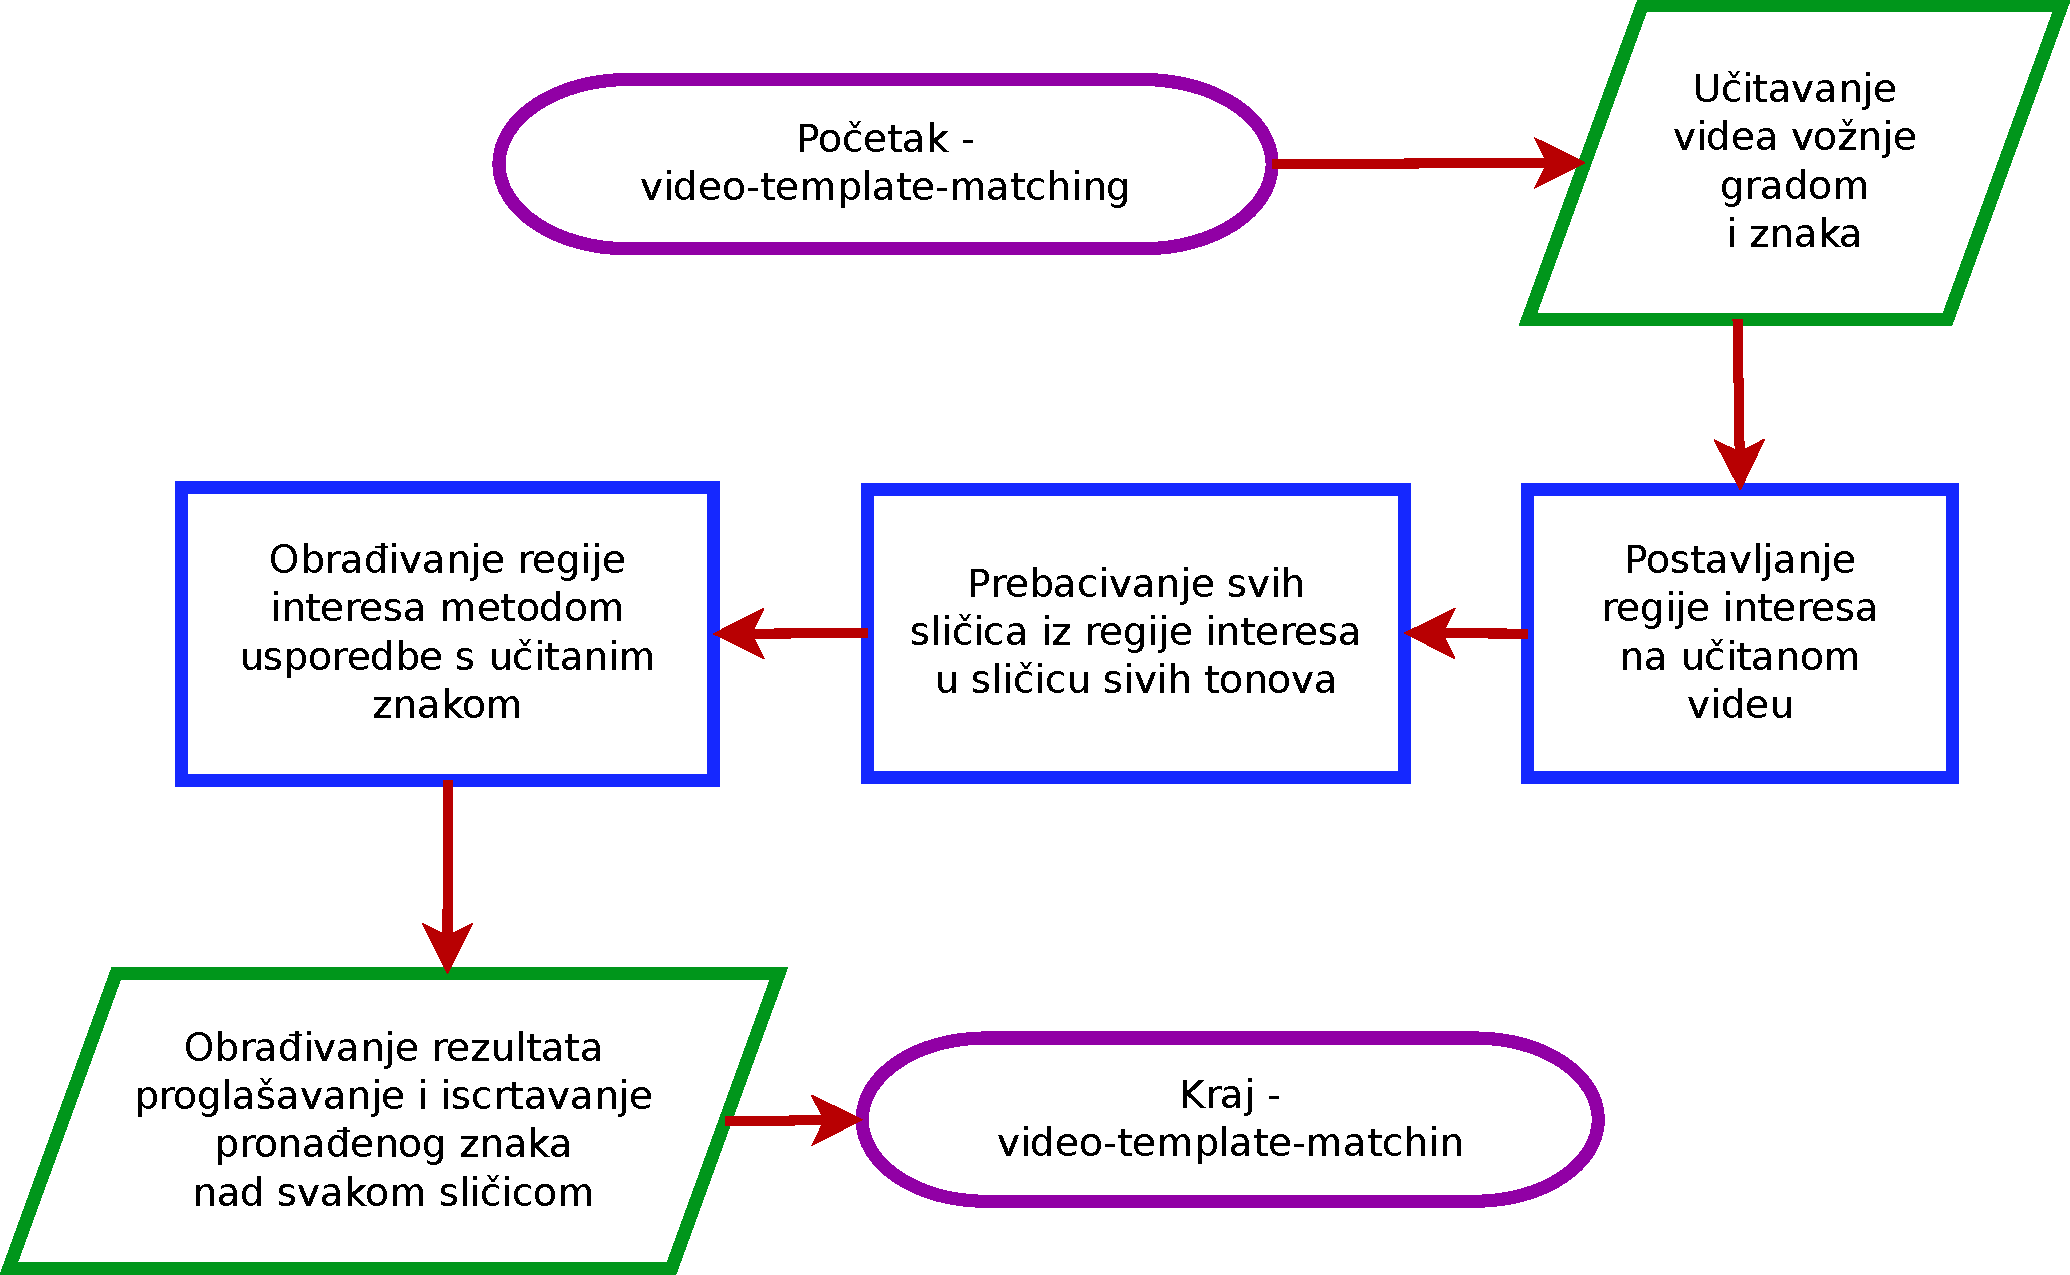
\includegraphics[scale=0.4]{figures/dijagramtoka.pdf}
\caption{Dijagram toka programa video-template-matching}
\label{fig:dijagramtoka.pdf}
\end{figure}


\newpage
\subsection{Učitavanje videa vožnje i učitavanje znaka} % (fold)
\label{ssub:Učitavanje videa vožnje i učitavanje znaka}

\begin{lstlisting}[label=lstUcit,caption={Izvorni kod za učitavanje
videa i znaka}]
#include "opencv2/imgproc/imgproc.hpp"

int main (int argc, char *argv[])
{
    // kreiranje objekta cap za ucitavanje videa
    VideoCapture cap("video/znakich2.mp4");
    if(!cap.isOpened())  // provjera uspjeha ucitavanja
        return -1;

    // kreiranje objekta Mat za spremanje znakova
    Mat znak1, znak2, znak3, znak4;

    // ucitavanje izrezanih znakova u razlicitim velicinama
    // trenutno se koristim samo znak2 
    znak1 = imread ("roi/01_roi.png");		
    znak2 = imread ("roi/02_roi.png");
    znak3 = imread ("roi/03_roi.png");
    znak4 = imread ("roi/04_roi.png");

    return 0;
}
\end{lstlisting}

Izlistanje koda~\ref{lstUcit} prikazuje primjer učitavanja videa i
učitavanje znaka upotrebom klase \texttt{VideoCapture} i funkcije
\texttt{imread} koji su uključeni dodavanjem biblioteke
\texttt{imgproc.hpp}. Kreiranom objektu \texttt{cap} predana je putanja
do videa kojeg treba učitati. Ukoliko video nije uspješno učitan program
završava i vraća \texttt{-1}. Kreiranim objektima \texttt{znak1},
\texttt{znak2}, \texttt{znak3}, \texttt{znak4} pridjeljene su slike
učitane upotrebom funkcije \texttt{imread} kojoj je predana putanja do
slike koju treba učitati.



% subsection Učitavanje videa vožnje i učitavanje znaka (end)


% section Prepoznavanje prometnog (end)
